\documentclass[../rapport_MVEX01-11-05]{subfiles}
\begin{document}

\subsection{Egenskaper}

\subsubsection{Observationer i egenskapsrumet}

\notes{förklara vilka som ser ut
att fungera bäst för att urskilja gester.}

Trots att gesterna ligger mycket tätt i egenskapsrummet (se
figur~\ref{fig:feats1011}) så är de mycket tydligt grupperade, vilket 
gör att \knn-metoden ger mycket exakta resultat.

\begin{figure}[htbp]
  \centering
  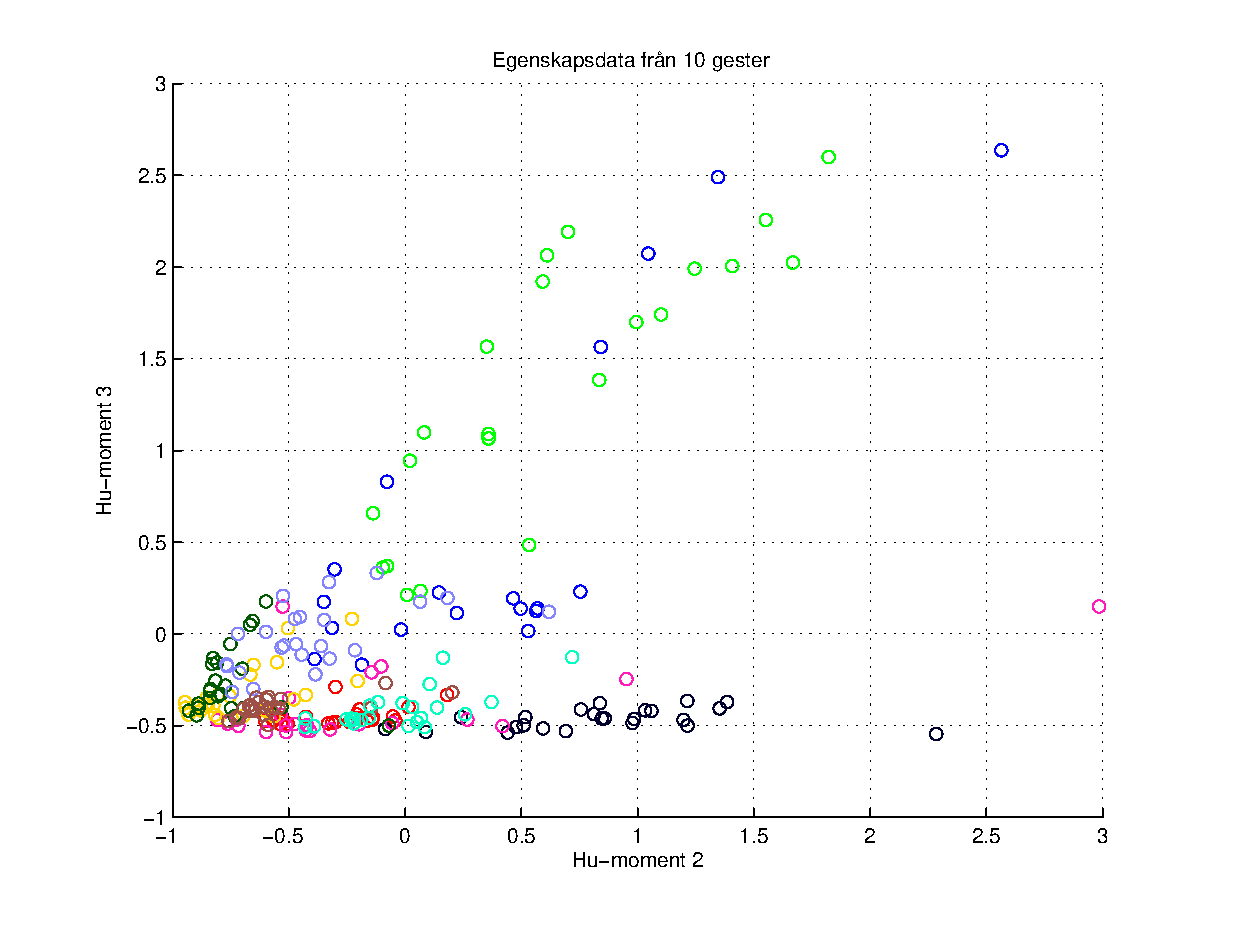
\includegraphics[width=\textwidth]{bilder/feats-10+11}
  \caption{Andra och tredje Hu-momenten för prototypdatan}
  \label{fig:feats1011}
\end{figure}

\end{document}